\documentclass{book}
\usepackage[a4paper,top=2.5cm,bottom=2.5cm,left=2.5cm,right=2.5cm]{geometry}
\usepackage{makeidx}
\usepackage{natbib}
\usepackage{graphicx}
\usepackage{multicol}
\usepackage{float}
\usepackage{listings}
\usepackage{color}
\usepackage{ifthen}
\usepackage[table]{xcolor}
\usepackage{textcomp}
\usepackage{alltt}
\usepackage{ifpdf}
\ifpdf
\usepackage[pdftex,
            pagebackref=true,
            colorlinks=true,
            linkcolor=blue,
            unicode
           ]{hyperref}
\else
\usepackage[ps2pdf,
            pagebackref=true,
            colorlinks=true,
            linkcolor=blue,
            unicode
           ]{hyperref}
\usepackage{pspicture}
\fi
\usepackage[utf8]{inputenc}
\usepackage{mathptmx}
\usepackage[scaled=.90]{helvet}
\usepackage{courier}
\usepackage{sectsty}
\usepackage{amssymb}
\usepackage[titles]{tocloft}
\usepackage{doxygen}
\lstset{language=C++,inputencoding=utf8,basicstyle=\footnotesize,breaklines=true,breakatwhitespace=true,tabsize=4,numbers=left }
\makeindex
\setcounter{tocdepth}{3}
\renewcommand{\footrulewidth}{0.4pt}
\renewcommand{\familydefault}{\sfdefault}
\hfuzz=15pt
\setlength{\emergencystretch}{15pt}
\hbadness=750
\tolerance=750
\begin{document}
\hypersetup{pageanchor=false,citecolor=blue}
\begin{titlepage}
\vspace*{7cm}
\begin{center}
{\Large Ambiente de Teste para Filtros Adaptativos }\\
\vspace*{1cm}
{\large Generated by Doxygen 1.8.3.1}\\
\vspace*{0.5cm}
{\small Mon Aug 5 2013 07:26:42}\\
\end{center}
\end{titlepage}
\clearemptydoublepage
\pagenumbering{roman}
\tableofcontents
\clearemptydoublepage
\pagenumbering{arabic}
\hypersetup{pageanchor=true,citecolor=blue}
\chapter{Class Index}
\section{Class List}
Here are the classes, structs, unions and interfaces with brief descriptions\-:\begin{DoxyCompactList}
\item\contentsline{section}{\hyperlink{classfoncfonc_1_1A}{foncfonc\-::\-A} }{\pageref{classfoncfonc_1_1A}}{}
\end{DoxyCompactList}

\chapter{File Index}
\section{\-File \-List}
\-Here is a list of all documented files with brief descriptions\-:\begin{DoxyCompactList}
\item\contentsline{section}{\hyperlink{main_8cpp}{main.\-cpp} }{\pageref{main_8cpp}}{}
\item\contentsline{section}{{\bfseries \-R\-E\-A\-D\-M\-E.\-md} }{\pageref{README_8md}}{}
\item\contentsline{section}{\hyperlink{Signal_8h}{\-Signal.\-h} }{\pageref{Signal_8h}}{}
\end{DoxyCompactList}

\chapter{Class Documentation}
\hypertarget{classfoncfonc_1_1A}{\section{foncfonc\-:\-:A Class Reference}
\label{classfoncfonc_1_1A}\index{foncfonc\-::\-A@{foncfonc\-::\-A}}
}
\subsection*{Public Attributes}
\begin{DoxyCompactItemize}
\item 
\hypertarget{classfoncfonc_1_1A_a54959ea2ab58000251776e0d819878f2}{int \hyperlink{classfoncfonc_1_1A_a54959ea2ab58000251776e0d819878f2}{x}}\label{classfoncfonc_1_1A_a54959ea2ab58000251776e0d819878f2}

\begin{DoxyCompactList}\small\item\em parâmetro escroto \end{DoxyCompactList}\end{DoxyCompactItemize}


\subsection{Detailed Description}
Classe zoada Um 

Definition at line 62 of file main.\-cpp.



The documentation for this class was generated from the following file\-:\begin{DoxyCompactItemize}
\item 
\hyperlink{main_8cpp}{main.\-cpp (no git)}\end{DoxyCompactItemize}

\chapter{File Documentation}
\hypertarget{main_8cpp}{\section{main.\-cpp File Reference}
\label{main_8cpp}\index{main.\-cpp@{main.\-cpp}}
}
{\ttfamily \#include $<$iostream$>$}\\*
Include dependency graph for main.\-cpp\-:\nopagebreak
\begin{figure}[H]
\begin{center}
\leavevmode
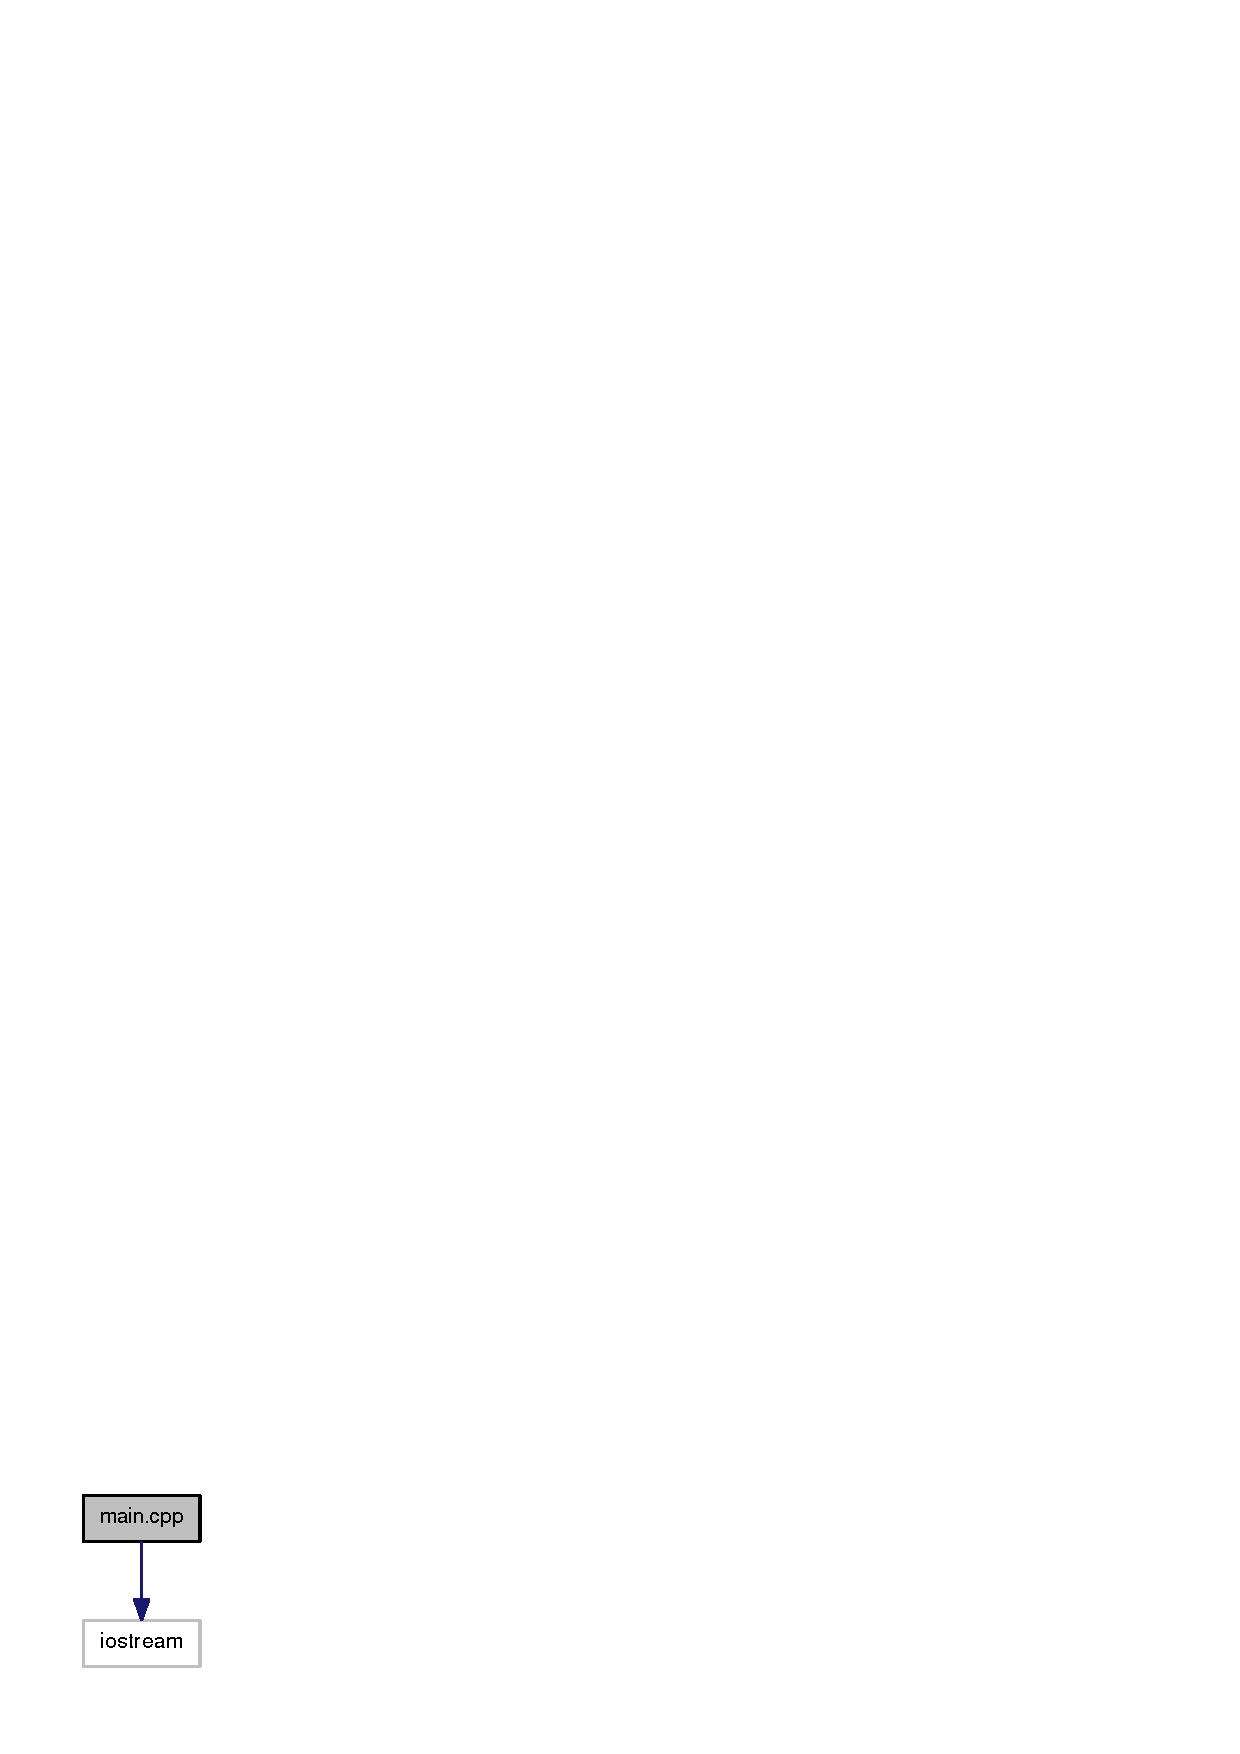
\includegraphics[width=136pt]{main_8cpp__incl}
\end{center}
\end{figure}
\subsection*{Classes}
\begin{DoxyCompactItemize}
\item 
class \hyperlink{classfoncfonc_1_1A}{foncfonc\-::\-A}
\end{DoxyCompactItemize}
\subsection*{Functions}
\begin{DoxyCompactItemize}
\item 
template typename$<$ T $>$ int \hyperlink{main_8cpp_aaaa9bbfe95c4caf7160980a028409f4c}{sgn} (T val, int zero=1)
\item 
int {\bfseries funcfunc\-::func1} (float x, int y)
\item 
int {\bfseries funcfunc\-::func2} (int x=4)
\item 
int \hyperlink{main_8cpp_a0ddf1224851353fc92bfbff6f499fa97}{main} (int argc, char $\ast$argv\mbox{[}$\,$\mbox{]})
\end{DoxyCompactItemize}


\subsection{Detailed Description}
Arquivo mêm ponto cê pê pê

\begin{DoxyAuthor}{Author}
Pedro Angelo Medeiros Fonini 
\end{DoxyAuthor}


Definition in file \hyperlink{main_8cpp_source}{main.\-cpp}.



\subsection{Function Documentation}
\hypertarget{main_8cpp_a0ddf1224851353fc92bfbff6f499fa97}{\index{main.\-cpp@{main.\-cpp}!main@{main}}
\index{main@{main}!main.cpp@{main.\-cpp}}
\subsubsection[{main}]{\setlength{\rightskip}{0pt plus 5cm}int main (
\begin{DoxyParamCaption}
\item[{int}]{argc, }
\item[{char $\ast$}]{argv\mbox{[}$\,$\mbox{]}}
\end{DoxyParamCaption}
)}}\label{main_8cpp_a0ddf1224851353fc92bfbff6f499fa97}
função main ué 
\begin{DoxyParams}[1]{Parameters}
\mbox{\tt in}  & {\em argc} & qtde de paradas \\
\hline
\mbox{\tt in}  & {\em argv} & paradas \\
\hline
\end{DoxyParams}
\begin{DoxyReturn}{Returns}
to the operational system 
\end{DoxyReturn}


Definition at line 76 of file main.\-cpp.

\hypertarget{main_8cpp_aaaa9bbfe95c4caf7160980a028409f4c}{\index{main.\-cpp@{main.\-cpp}!sgn@{sgn}}
\index{sgn@{sgn}!main.cpp@{main.\-cpp}}
\subsubsection[{sgn}]{\setlength{\rightskip}{0pt plus 5cm}template typename$<$T$>$ int sgn (
\begin{DoxyParamCaption}
\item[{T}]{val, }
\item[{int}]{zero = {\ttfamily 1}}
\end{DoxyParamCaption}
)}}\label{main_8cpp_aaaa9bbfe95c4caf7160980a028409f4c}
Função irada que dá o sinal da variável. 
\begin{DoxyParams}[1]{Parameters}
\mbox{\tt in}  & {\em val} & val se fuder \\
\hline
\mbox{\tt in}  & {\em zero} & zero? \\
\hline
\end{DoxyParams}
\begin{DoxyReturn}{Returns}
to the caller 
\end{DoxyReturn}


Definition at line 34 of file main.\-cpp.


\addcontentsline{toc}{part}{Index}
\printindex
\end{document}
